\section{Impact of Autoencoder Architecture on In-Between Instance Preservation} \label{sec:rq1}

\begin{table}[htb]
\centering
\renewcommand\cellalign{cc}
\renewcommand\theadalign{cc}

% ----- First Table -----
\begin{subtable}[t]{\textwidth}
\centering
\begin{tabular}{|
  >{\centering\arraybackslash}m{0.15cm} |
  >{\centering\arraybackslash}m{0.50cm} |
  >{\centering\arraybackslash}m{2.00cm} |
  >{\centering\arraybackslash}m{2.33cm} |
  >{\centering\arraybackslash}m{2.66cm} |
  >{\centering\arraybackslash}m{3.00cm} |}
  \hline
  & & \multicolumn{4}{c|}{Network Depth} \\
  \hline
  & & \textbf{0} & \textbf{1} & \textbf{2} & \textbf{3} \\
  \hline
  \multirow{7}{*}{\rotatebox[origin=c]{90}{\parbox[c][0.15cm][c]{4.5cm}{\centering Network Width}}} 
    & \boldmath{$2^0$} 
    & \makecell{\textcolor{red!60!black}{0.1449} \\ \textit{2-1}} 
    & \makecell{\textcolor{red!100!black}{0.1458} \\ \textit{2-1-1}} 
    & \makecell{\textcolor{red!80!black}{0.1453} \\ \textit{2-2-1-1}} 
    & \makecell{0.0063 \\ \textit{2-4-2-1-1}} \\
  \cline{2-6}
  & \boldmath{$2^1$} 
    &  
    & \makecell{\textcolor{red!40!black}{0.0641} \\ \textit{2-2-1}} 
    & \makecell{\textcolor{red!20!black}{0.0374} \\ \textit{2-4-2-1}} 
    & \makecell{\textcolor{green!60!black}{0.0019} \\ \textit{2-8-4-2-1}} \\
  \cline{2-6}
  & \boldmath{$2^2$} 
    &  
    & \makecell{0.0171 \\ \textit{2-4-1}} 
    & \makecell{0.0094 \\ \textit{2-8-4-1}} 
    & \makecell{\textcolor{green!40!black}{0.0020} \\ \textit{2-16-8-4-1}} \\
  \cline{2-6}
  & \boldmath{$2^3$} 
    &  
    & \makecell{0.0049 \\ \textit{2-8-1}} 
    & \makecell{\textcolor{green!80!black}{0.0017} \\ \textit{2-16-8-1}} 
    & \makecell{\textcolor{green!100!black}{0.0016} \\ \textit{2-32-16-8-1}} \\
  \cline{2-6}
  & \boldmath{$2^4$} 
    &  
    & \makecell{0.0036 \\ \textit{2-16-1}} 
    & \makecell{\textcolor{green!60!black}{0.0019} \\ \textit{2-32-16-1}} 
    & \makecell{\textcolor{green!40!black}{0.0020} \\ \textit{2-64-32-16-1}} \\
  \cline{2-6}
  & \boldmath{$2^5$} 
    &  
    & \makecell{\textcolor{green!20!black}{0.0026} \\ \textit{2-32-1}} 
    & \makecell{\textcolor{green!60!black}{0.0019} \\ \textit{2-64-32-1}} 
    & \makecell{\textcolor{green!20!black}{0.0026} \\ \textit{2-128-64-32-1}} \\
  \hline
\end{tabular}
\caption{2D autoencoder.}
\label{tab:rq1-2d}
\end{subtable}

\vspace{1em} % spacing between tables

% ----- Second Table -----
\begin{subtable}[t]{\textwidth}
\centering
\begin{tabular}{|
  >{\centering\arraybackslash}m{0.15cm} |
  >{\centering\arraybackslash}m{0.50cm} |
  >{\centering\arraybackslash}m{2.00cm} |
  >{\centering\arraybackslash}m{2.33cm} |
  >{\centering\arraybackslash}m{2.66cm} |
  >{\centering\arraybackslash}m{3.00cm} |}
  \hline
  & & \multicolumn{4}{c|}{Network Depth} \\
  \hline
  & & \textbf{0} & \textbf{1} & \textbf{2} & \textbf{3} \\
  \hline
  \multirow{7}{*}{\rotatebox[origin=c]{90}{\parbox[c][0.15cm][c]{5.5cm}{\centering Network Width}}} 
    & \boldmath{$2^0$} 
    & \makecell{\textcolor{red!40!black}{2.1619} \\ \textit{3-2}} 
    & \makecell{\textcolor{red!100!black}{4.3859} \\ \textit{3-1-2}} 
    & \makecell{\textcolor{red!80!black}{3.4299} \\ \textit{3-2-1-2}} 
    & \makecell{\textcolor{red!20!black}{2.1483} \\ \textit{3-4-2-1-2}} \\
  \cline{2-6}
  & \boldmath{$2^1$} 
    &  
    & \makecell{\textcolor{red!60!black}{2.1625} \\ \textit{3-2-2}} 
    & \makecell{0.6318 \\ \textit{3-4-2-2}} 
    & \makecell{0.2784 \\ \textit{3-8-4-2-2}} \\
  \cline{2-6}
  & \boldmath{$2^2$} 
    &  
    & \makecell{0.5070 \\ \textit{3-4-2}} 
    & \makecell{0.2157 \\ \textit{3-8-4-2}} 
    & \makecell{0.1488 \\ \textit{3-16-8-4-2}} \\
  \cline{2-6}
  & \boldmath{$2^3$} 
    &  
    & \makecell{0.3851 \\ \textit{3-8-2}} 
    & \makecell{0.1397 \\ \textit{3-16-8-2}} 
    & \makecell{\textcolor{green!40!black}{0.1116} \\ \textit{3-32-16-8-2}} \\
  \cline{2-6}
  & \boldmath{$2^4$} 
    &  
    & \makecell{0.2232 \\ \textit{3-16-2}} 
    & \makecell{\textcolor{green!60!black}{0.1018} \\ \textit{3-32-16-2}} 
    & \makecell{\textcolor{green!100!black}{0.0920} \\ \textit{3-64-32-16-2}} \\  
  \cline{2-6}
  & \boldmath{$2^5$} 
    &  
    & \makecell{0.1696 \\ \textit{3-32-2}} 
    & \makecell{\textcolor{green!80!black}{0.0936} \\ \textit{3-64-32-2}} 
    & \makecell{\textcolor{green!20!black}{0.1131} \\ \textit{3-128-64-32-2}} \\
  \hline
\end{tabular}
\caption{3D autoencoder.}
\label{tab:rq1-3d}
\end{subtable}

% ----- Main Caption -----
\caption{Grid search results across 2D and 3D autoencoders. Each cell displays the mean squared error (MSE) loss (top) and the corresponding encoder architecture (bottom). Network width indicates the number of units in the first layer both before and after the bottleneck, and network depth refers to the number of hidden layers in the encoder. The top and worst 5 results are visually highlighted.}
\label{tab:rq1-combined}
\end{table}

\begin{figure}[htb]
    \centering
    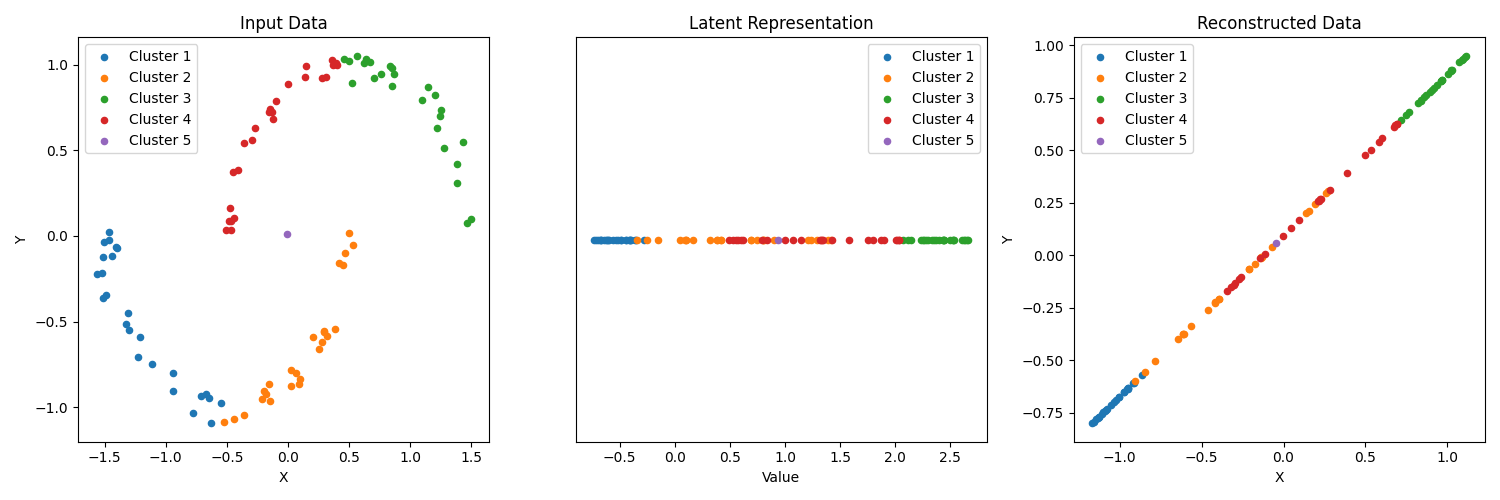
\includegraphics[width=\linewidth]{images/RQ1/2-1_0.1449.png}
    \caption{Baseline projections for a 2D autoencoder with no hidden layers (2–1 architecture) and \textcolor{red!60!black}{0.1449} MSE. This linear mapping serves as a reference.}
    \label{fig:2-1}
\end{figure}

\begin{figure}[htb]
  \centering
  % subfigure 1
  \begin{subfigure}[b]{0.49\textwidth}
    \centering
    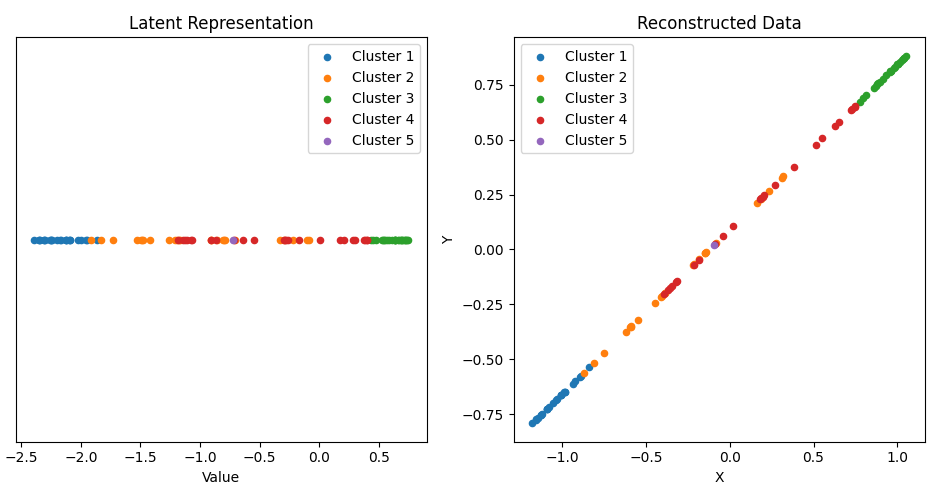
\includegraphics[width=\linewidth]{images/RQ1/2-1-1_0.1458.png}
    \caption{2-1-1 architecture with \textcolor{red!100!black}{0.1458} MSE.}
    \label{fig:2-1-1}
  \end{subfigure}
  \hfill
  % subfigure 2
  \begin{subfigure}[b]{0.49\textwidth}
    \centering
    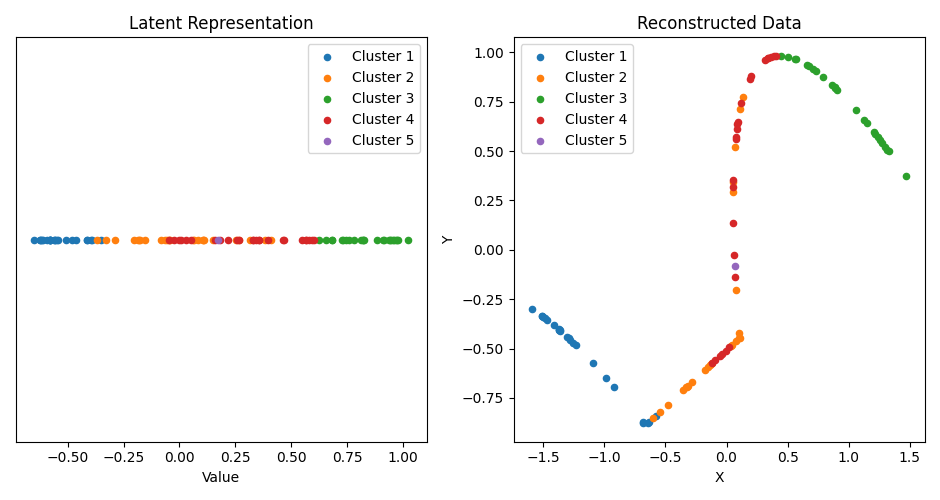
\includegraphics[width=\linewidth]{images/RQ1/2-2-1_0.0641.png}
    \caption{2-2-1 architecture with \textcolor{red!40!black}{0.0641} MSE.}
    \label{fig:2-2-1}
  \end{subfigure}
  \hfill
  % subfigure 3
  \begin{subfigure}[b]{0.49\textwidth}
    \centering
    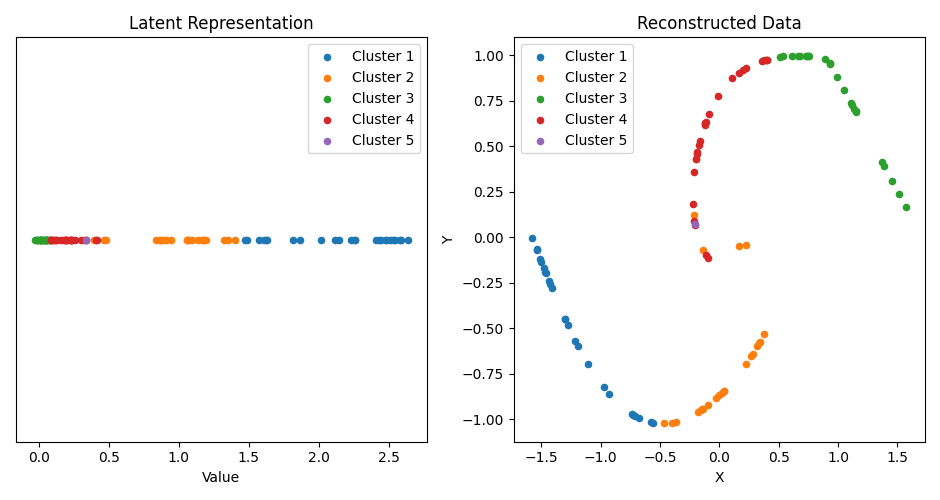
\includegraphics[width=\linewidth]{images/RQ1/2-4-1_0.0171.png}
    \caption{2-4-1 architecture with 0.0171 MSE.}
    \label{fig:2-4-1}
  \end{subfigure}
  \hfill
  % subfigure 4
  \begin{subfigure}[b]{0.49\textwidth}
    \centering
    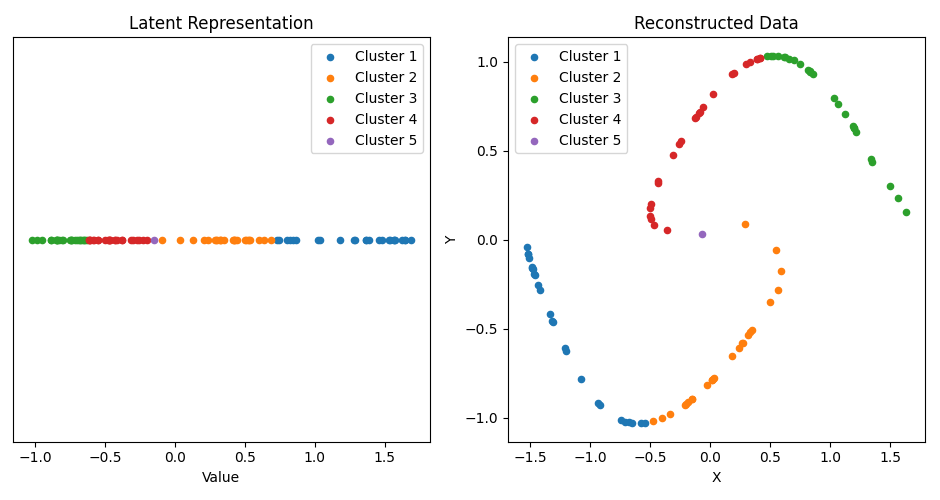
\includegraphics[width=\linewidth]{images/RQ1/2-8-1_0.0049.png}
    \caption{2-8-1 architecture with 0.0049 MSE.}
    \label{fig:2-8-1}
  \end{subfigure}
  \hfill
  % subfigure 5
  \begin{subfigure}[b]{0.49\textwidth}
    \centering
    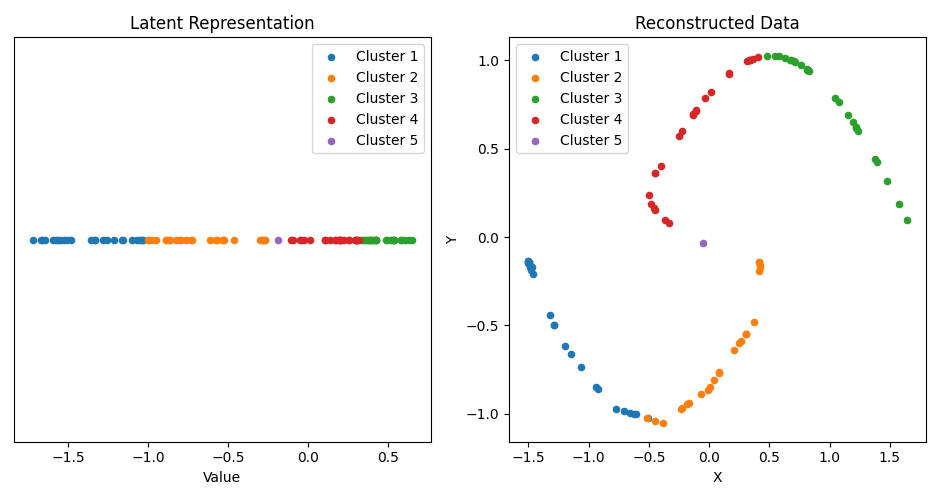
\includegraphics[width=\linewidth]{images/RQ1/2-16-1_0.0036.png}
    \caption{2-16-1 architecture with 0.0036 MSE.}
    \label{fig:2-16-1}
  \end{subfigure}
  \hfill
  % subfigure 6
  \begin{subfigure}[b]{0.49\textwidth}
    \centering
    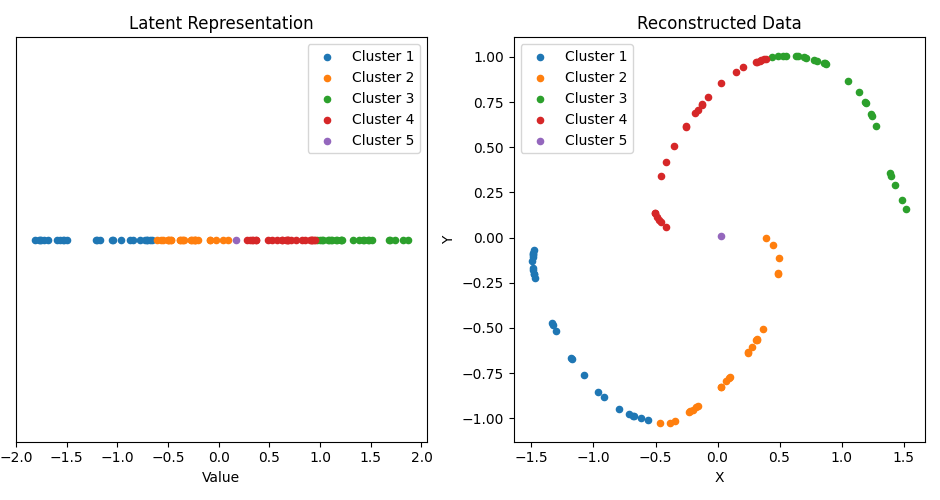
\includegraphics[width=\linewidth]{images/RQ1/2-32-1_0.0026.png}
    \caption{2-32-1 architecture with \textcolor{green!20!black}{0.0026} MSE.}
    \label{fig:2-32-1}
  \end{subfigure}

  \caption{Projections for 2D autoencoders with a single hidden layer of varying width. 2-X-1 architectures are compared.}
  \label{fig:2-X-1}
\end{figure}

\begin{figure}[htb]
  \centering
  % subfigure 1
  \begin{subfigure}[b]{0.49\textwidth}
    \centering
    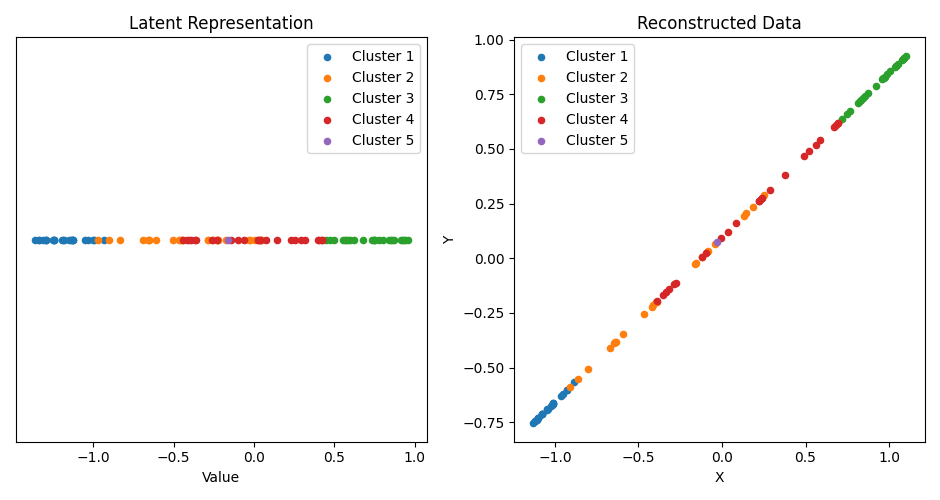
\includegraphics[width=\linewidth]{images/RQ1/2-2-1-1_0.1453.png}
    \caption{2-2-1-1 architecture with \textcolor{red!80!black}{0.1453} MSE.}
    \label{fig:2-2-1-1-2}
  \end{subfigure}
  \hfill
  % subfigure 2
  \begin{subfigure}[b]{0.49\textwidth}
    \centering
    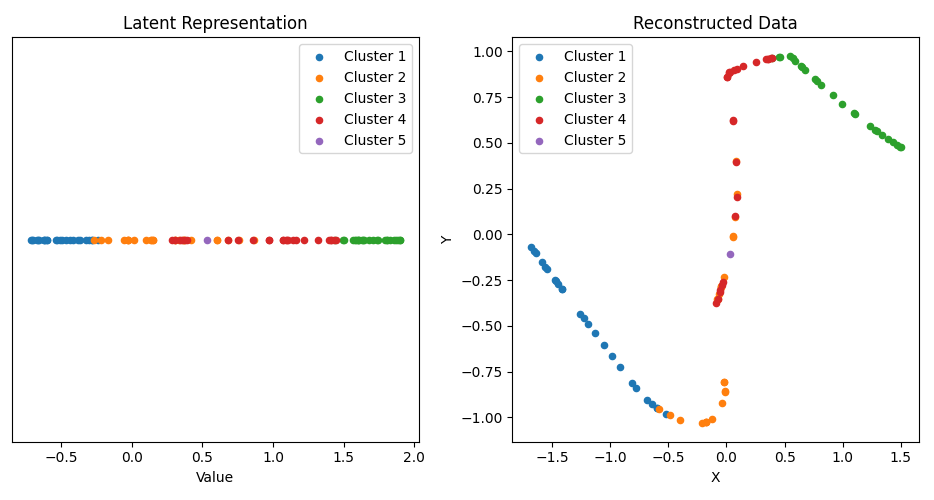
\includegraphics[width=\linewidth]{images/RQ1/2-4-2-1_0.0374.png}
    \caption{2-4-2-1 architecture with \textcolor{red!20!black}{0.0374} MSE.}
    \label{fig:2-4-2-1}
  \end{subfigure}
  \hfill
  % subfigure 3
  \begin{subfigure}[b]{0.49\textwidth}
    \centering
    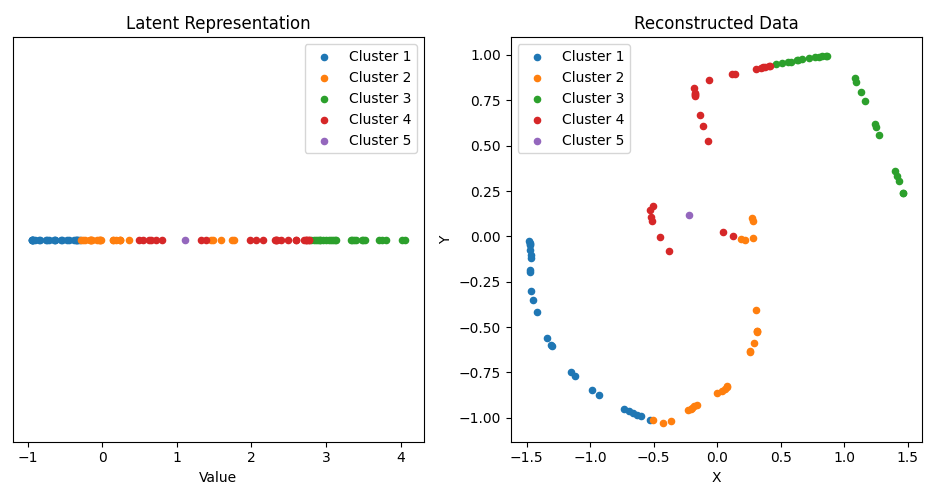
\includegraphics[width=\linewidth]{images/RQ1/2-8-4-1_0.0094.png}
    \caption{2-8-4-1 architecture with 0.0094 MSE.}
    \label{fig:2-8-4-1}
  \end{subfigure}
  \hfill
  % subfigure 4
  \begin{subfigure}[b]{0.49\textwidth}
    \centering
    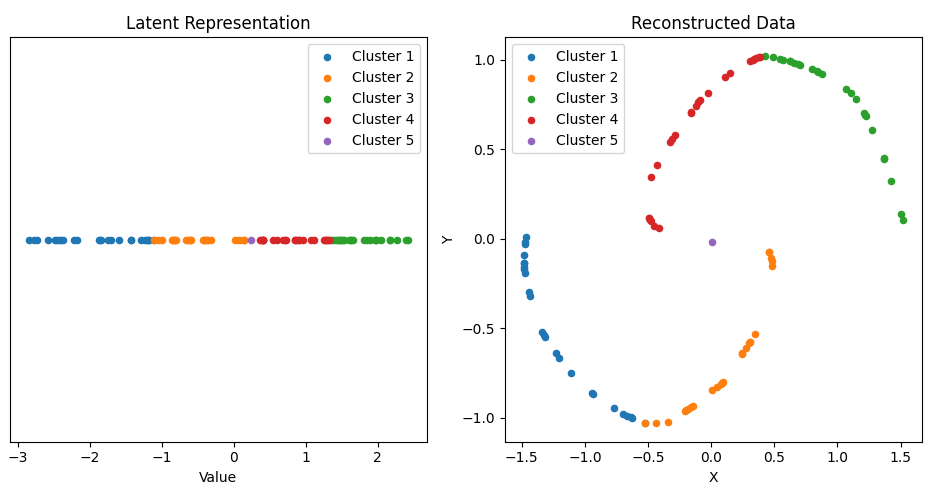
\includegraphics[width=\linewidth]{images/RQ1/2-16-8-1_0.0017.png}
    \caption{2-16-8-1 architecture with \textcolor{green!80!black}{0.0017} MSE.}
    \label{fig:2-16-8-1}
  \end{subfigure}
  \hfill
  % subfigure 5
  \begin{subfigure}[b]{0.49\textwidth}
    \centering
    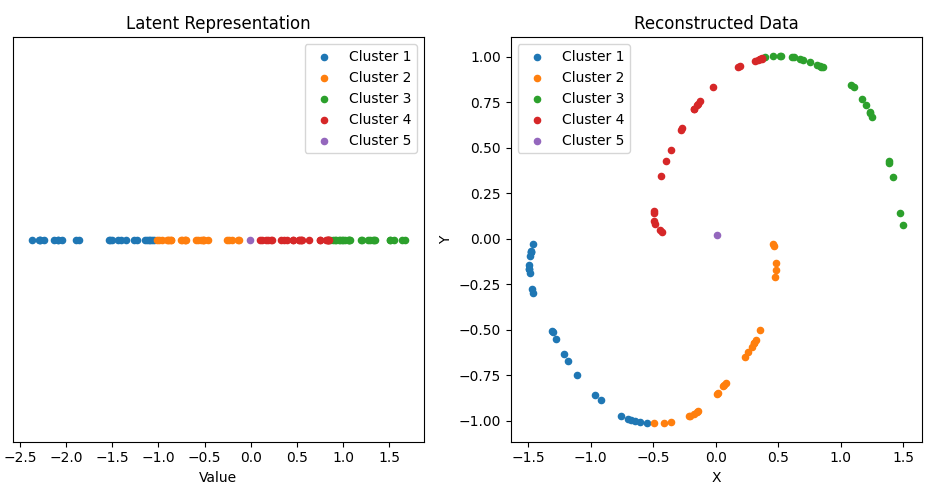
\includegraphics[width=\linewidth]{images/RQ1/2-32-16-1_0.0019.png}
    \caption{2-32-16-1 architecture with \textcolor{green!60!black}{0.0019} MSE.}
    \label{fig:2-32-16-1}
  \end{subfigure}
  \hfill
  % subfigure 6
  \begin{subfigure}[b]{0.49\textwidth}
    \centering
    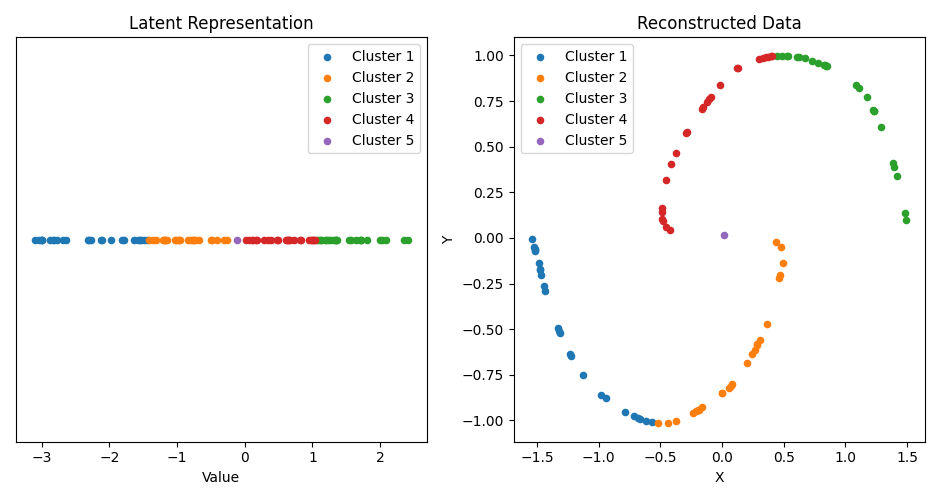
\includegraphics[width=\linewidth]{images/RQ1/2-64-32-1_0.0019.png}
    \caption{2-64-32-1 architecture with \textcolor{green!60!black}{0.0019} MSE.}
    \label{fig:2-64-32-1}
  \end{subfigure}

  \caption{Projections for 2D autoencoders with two hidden layers of varying width. 2-X-Y-1 architectures are compared.}
  \label{fig:2-X-Y-1}
\end{figure}

\begin{figure}[htb]
  \centering
  % subfigure 1
  \begin{subfigure}[b]{0.49\textwidth}
    \centering
    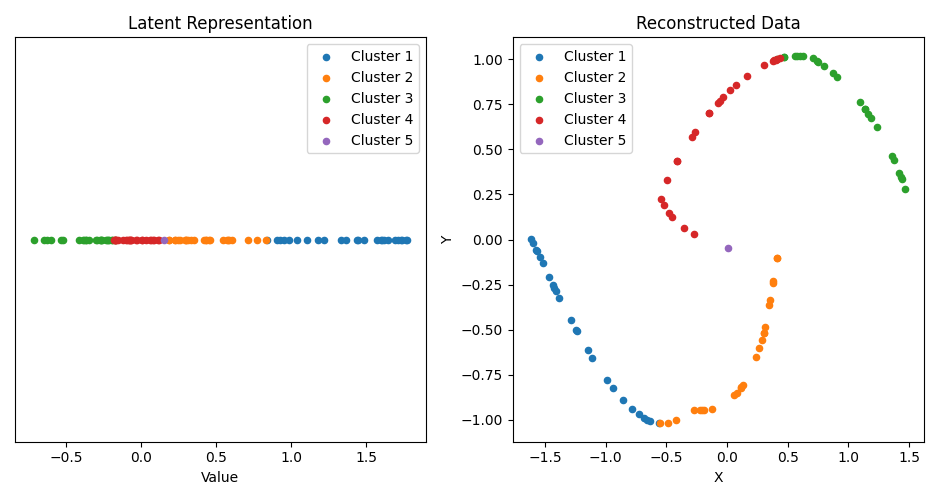
\includegraphics[width=\linewidth]{images/RQ1/2-4-2-1-1_0.0063.png}
    \caption{2-4-2-1-1 architecture with 0.0063 MSE.}
    \label{fig:2-4-2-1-1}
  \end{subfigure}
  \hfill
  % subfigure 2
  \begin{subfigure}[b]{0.49\textwidth}
    \centering
    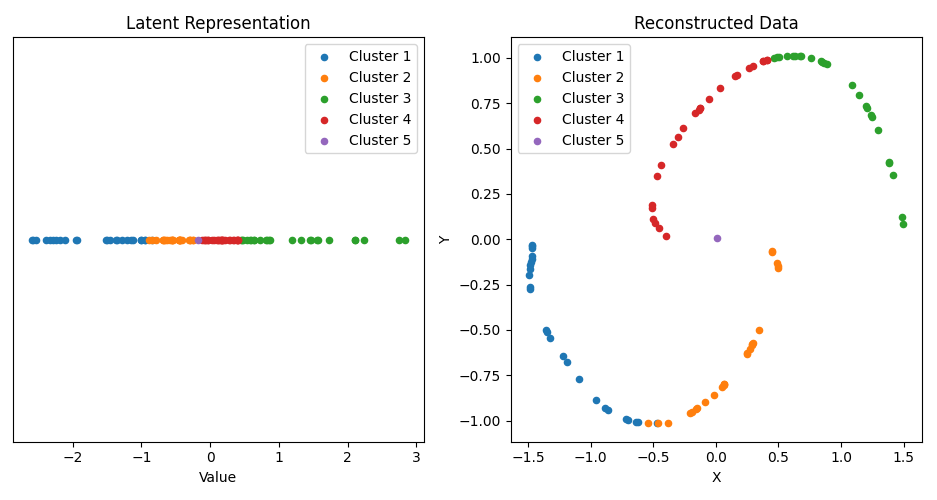
\includegraphics[width=\linewidth]{images/RQ1/2-8-4-2-1_0.0019.png}
    \caption{2-8-4-2-1 architecture with \textcolor{green!60!black}{0.0019} MSE.}
    \label{fig:2-8-4-2-1}
  \end{subfigure}
  \hfill
  % subfigure 3
  \begin{subfigure}[b]{0.49\textwidth}
    \centering
    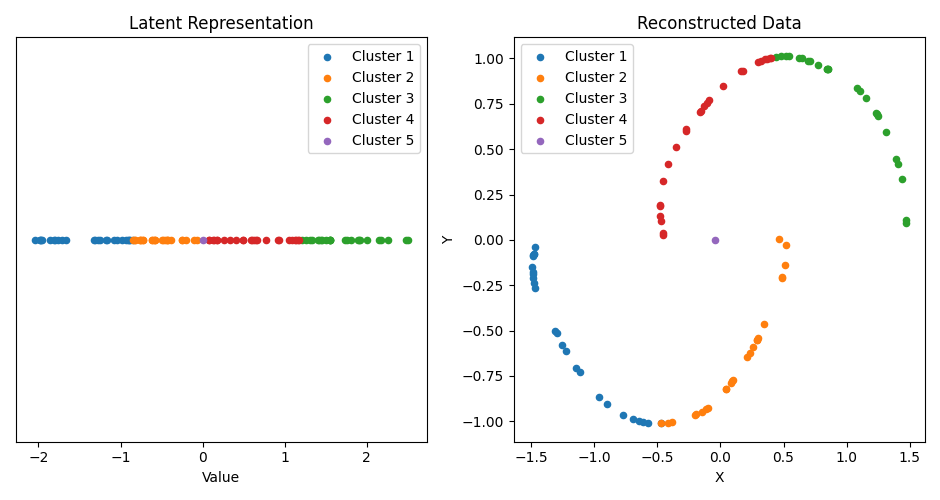
\includegraphics[width=\linewidth]{images/RQ1/2-16-8-4-1_0.0020.png}
    \caption{2-16-8-4-1 architecture with \textcolor{green!40!black}{0.0020} MSE.}
    \label{fig:2-16-8-4-1}
  \end{subfigure}
  \hfill
  % subfigure 4
  \begin{subfigure}[b]{0.49\textwidth}
    \centering
    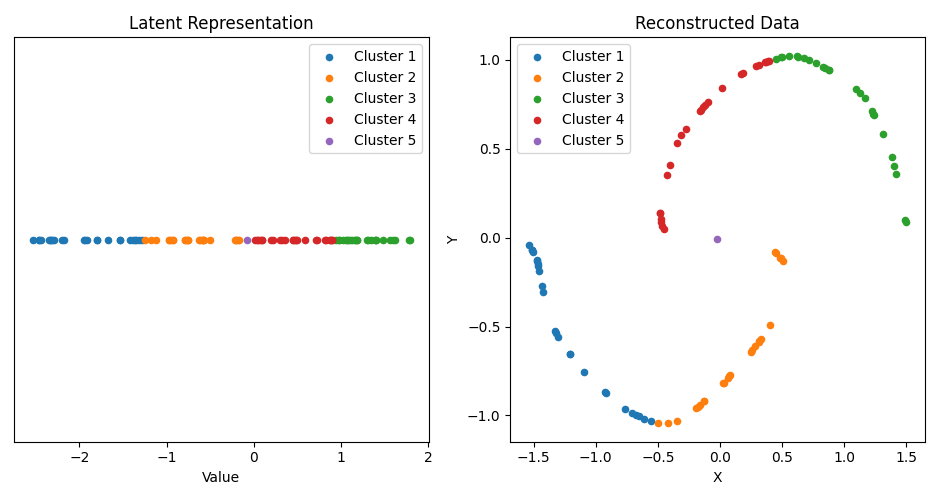
\includegraphics[width=\linewidth]{images/RQ1/2-32-16-8-1_0.0016.png}
    \caption{2-32-16-8-1 architecture with \textcolor{green!100!black}{0.0016} MSE.}
    \label{fig:2-32-16-8-1}
  \end{subfigure}
  \hfill
  % subfigure 5
  \begin{subfigure}[b]{0.49\textwidth}
    \centering
    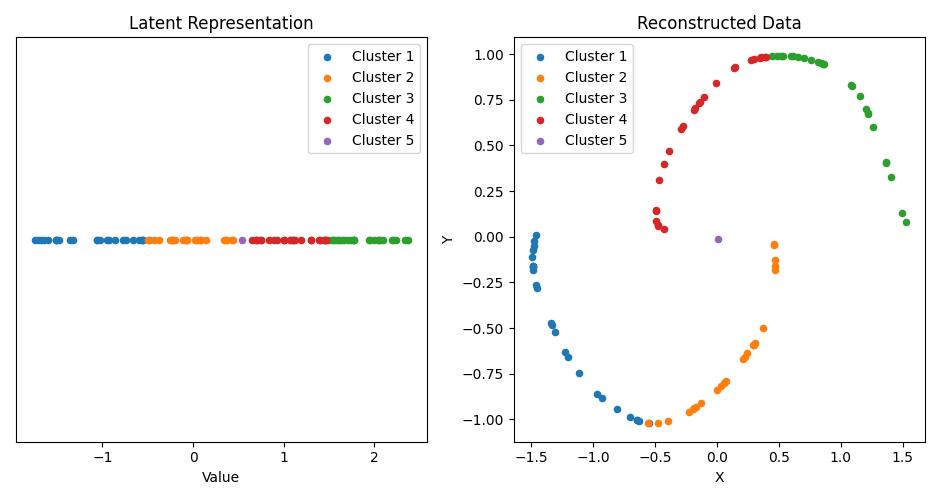
\includegraphics[width=\linewidth]{images/RQ1/2-64-32-16-1_0.0020.png}
    \caption{2-64-32-16-1 architecture with \textcolor{green!40!black}{0.0020} MSE.}
    \label{fig:2-64-32-16-1}
  \end{subfigure}
  \hfill
  % subfigure 6
  \begin{subfigure}[b]{0.49\textwidth}
    \centering
    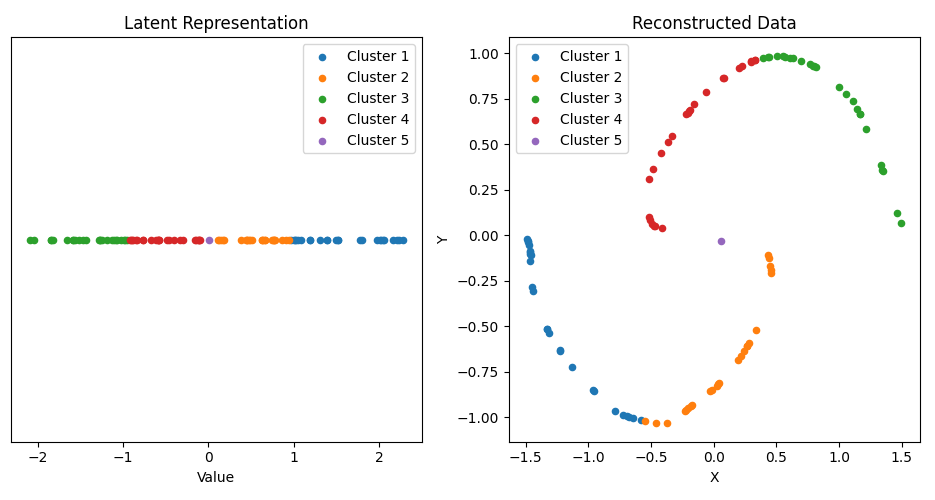
\includegraphics[width=\linewidth]{images/RQ1/2-128-64-32-1_0.0026.png}
    \caption{2-128-64-32-1 architecture with \textcolor{green!20!black}{0.0026} MSE.}
    \label{fig:2-128-64-32-1}
  \end{subfigure}

  \caption{Projections for 2D autoencoders with three hidden layers of varying width. 2-X-Y-Z-1 architectures are compared.}
  \label{fig:2-X-Y-Z-1}
\end{figure}

\begin{figure}[htb]
    \centering
    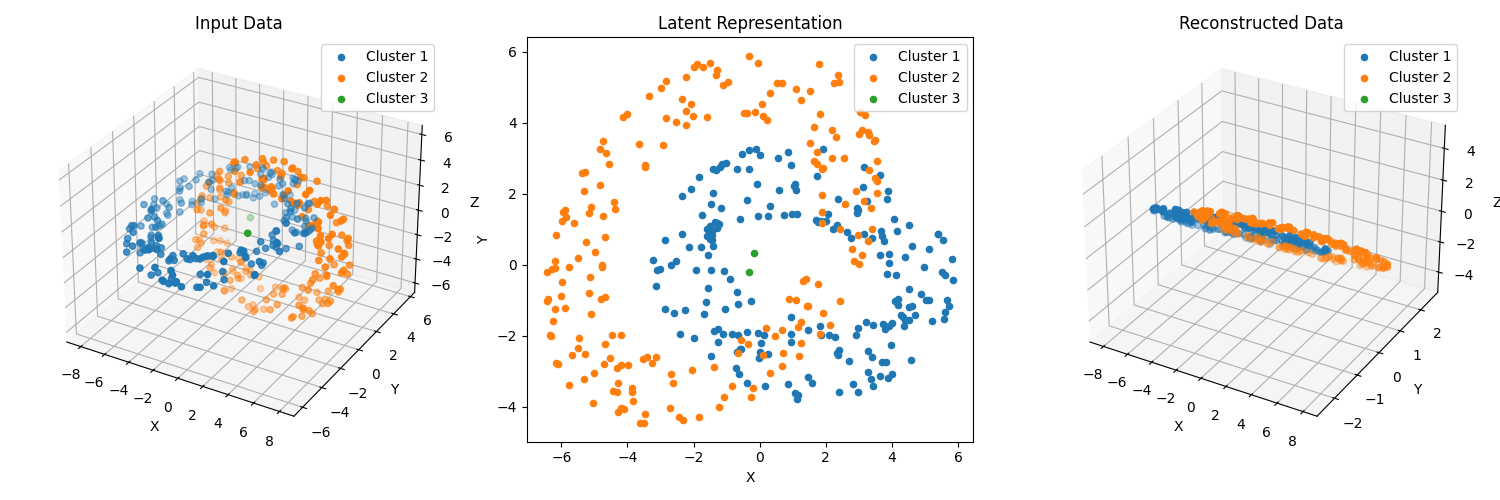
\includegraphics[width=\linewidth]{images/RQ1/3-2_2.1619.png}
    \caption{Baseline projections for a 3D autoencoder with no hidden layers (3–2 architecture) and \textcolor{red!40!black}{2.1619} MSE. This linear mapping serves as a reference.}
    \label{fig:3-2}
\end{figure}

\begin{figure}[htb]
  \centering
  % subfigure 1
  \begin{subfigure}[b]{0.49\textwidth}
    \centering
    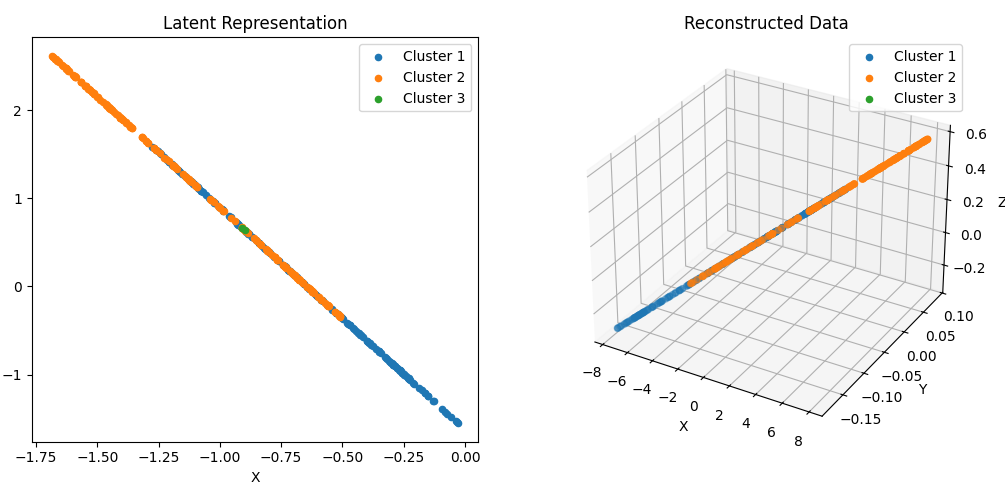
\includegraphics[width=\linewidth]{images/RQ1/3-1-2_4.3859.png}
    \caption{3-1-2 architecture with \textcolor{red!100!black}{4.3859} MSE.}
    \label{fig:3-1-2}
  \end{subfigure}
  \hfill
  % subfigure 2
  \begin{subfigure}[b]{0.49\textwidth}
    \centering
    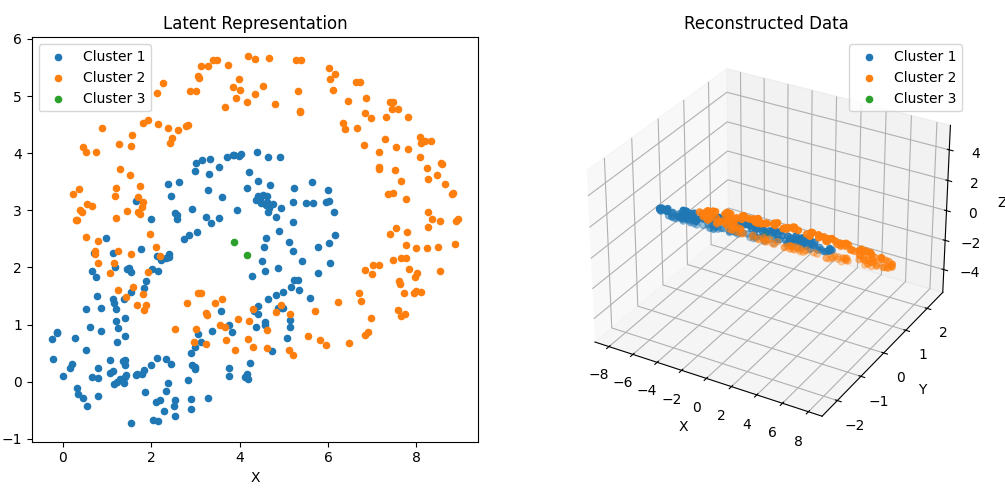
\includegraphics[width=\linewidth]{images/RQ1/3-2-2_2.1625.png}
    \caption{3-2-2 architecture with \textcolor{red!60!black}{2.1625} MSE.}
    \label{fig:3-2-2}
  \end{subfigure}
  \hfill
  % subfigure 3
  \begin{subfigure}[b]{0.49\textwidth}
    \centering
    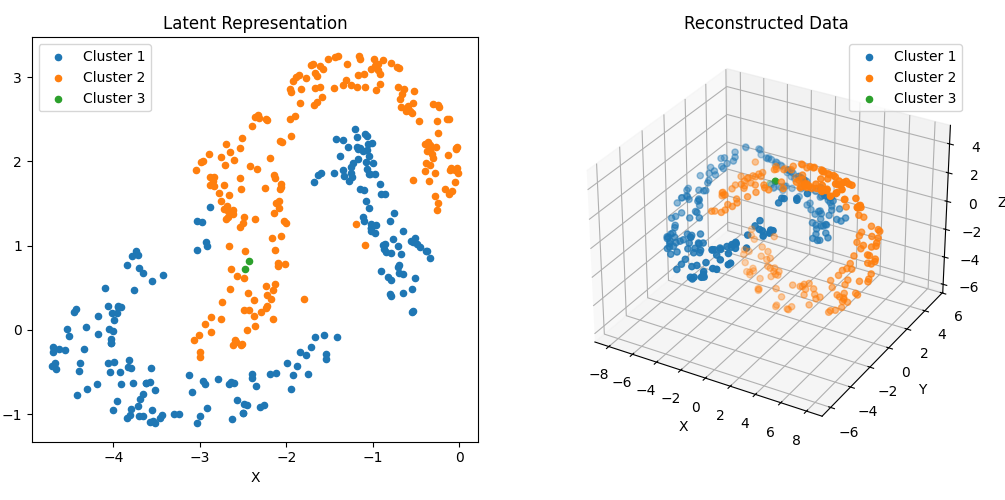
\includegraphics[width=\linewidth]{images/RQ1/3-4-2_0.5070.png}
    \caption{3-4-2 architecture with 0.5070 MSE.}
    \label{fig:3-4-2}
  \end{subfigure}
  \hfill
  % subfigure 4
  \begin{subfigure}[b]{0.49\textwidth}
    \centering
    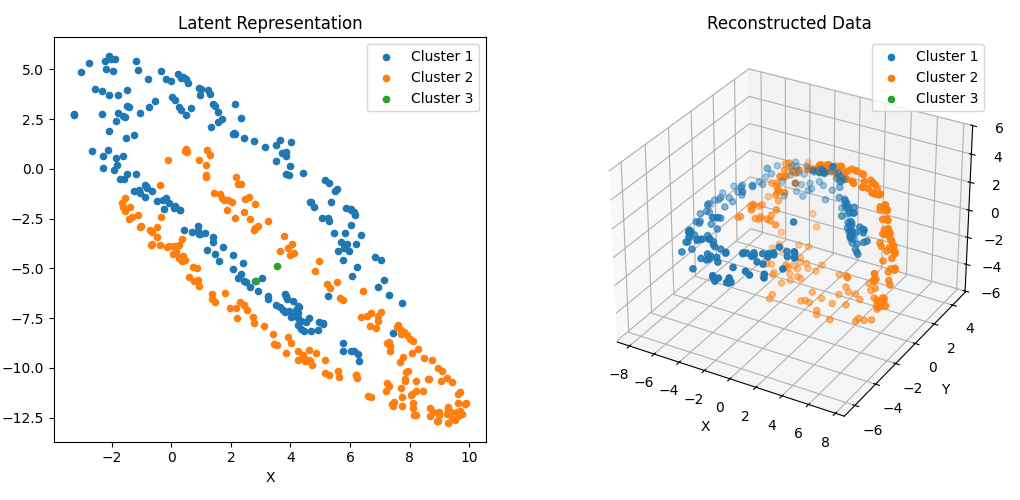
\includegraphics[width=\linewidth]{images/RQ1/3-8-2_0.3851.png}
    \caption{3-8-2 architecture with 0.3851 MSE.}
    \label{fig:3-8-2}
  \end{subfigure}
  \hfill  
  % subfigure 5
  \begin{subfigure}[b]{0.49\textwidth}
    \centering
    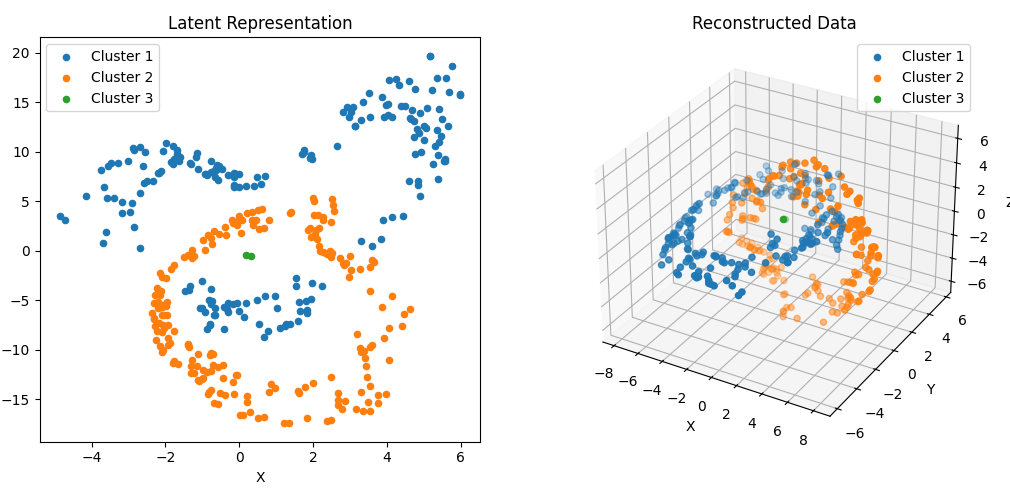
\includegraphics[width=\linewidth]{images/RQ1/3-16-2_0.2232.png}
    \caption{3-16-2 architecture with 0.2232 MSE.}
    \label{fig:3-16-2}
  \end{subfigure}
  \hfill  
  % subfigure 6
  \begin{subfigure}[b]{0.49\textwidth}
    \centering
    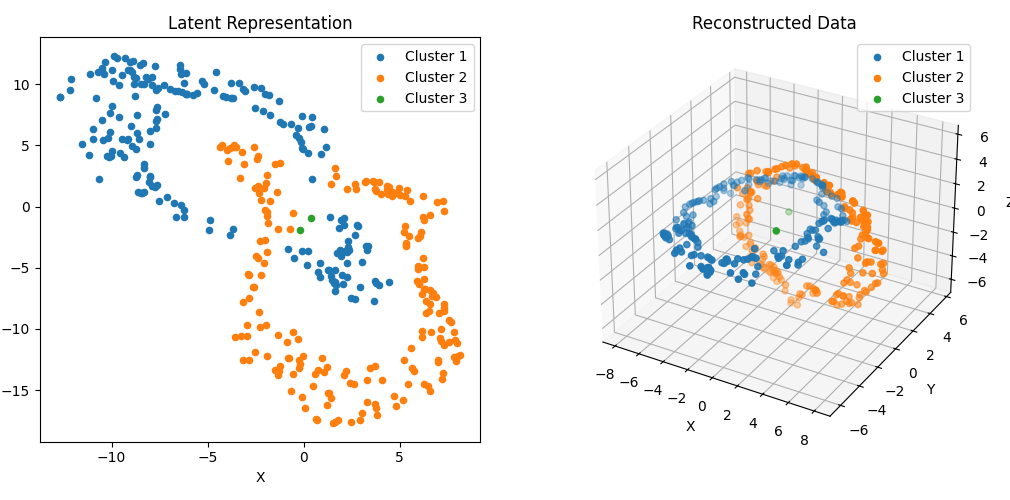
\includegraphics[width=\linewidth]{images/RQ1/3-32-2_0.1696.png}
    \caption{3-32-2 architecture with 0.1696 MSE.}
    \label{fig:3-32-2}
  \end{subfigure}

  \caption{Projections for 3D autoencoders with one hidden layer of varying width. 3-X-2 architectures are compared.}
  \label{fig:3-X-2}
\end{figure}

\begin{figure}[htb]
  \centering
  % subfigure 1
  \begin{subfigure}[b]{0.49\textwidth}
    \centering
    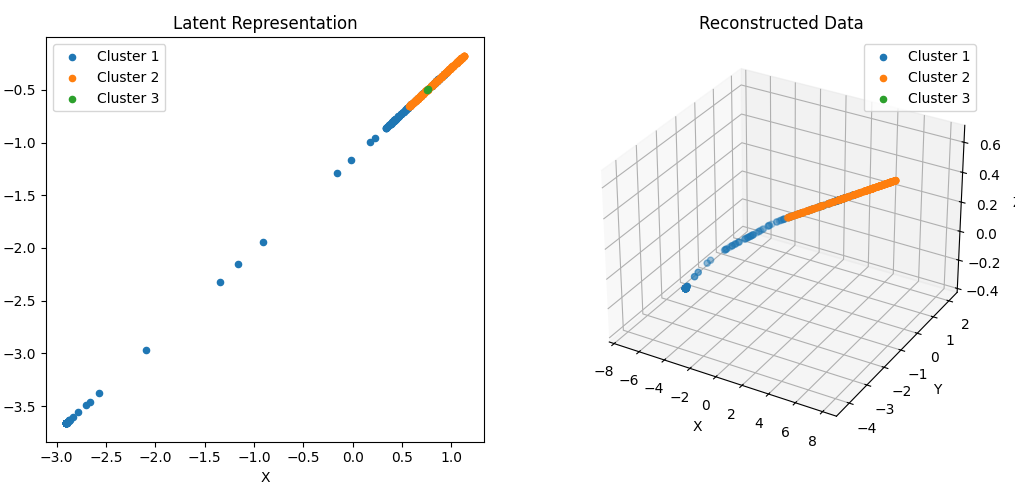
\includegraphics[width=\linewidth]{images/RQ1/3-2-1-2_3.4299.png}
    \caption{3-2-1-2 architecture with \textcolor{red!80!black}{3.4299} MSE.}
    \label{fig:3-2-1-2}
  \end{subfigure}
  \hfill
  % subfigure 2
  \begin{subfigure}[b]{0.49\textwidth}
    \centering
    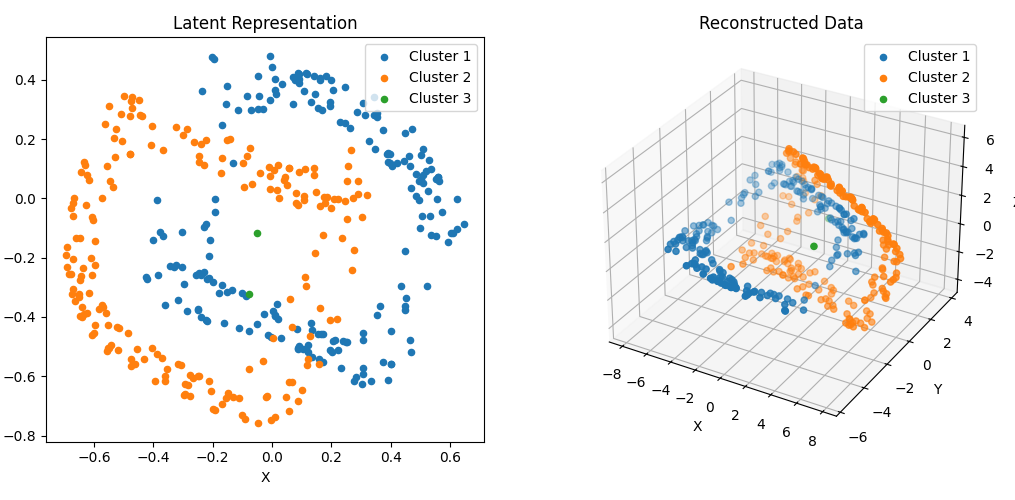
\includegraphics[width=\linewidth]{images/RQ1/3-4-2-2_0.6318.png}
    \caption{3-4-2-2 architecture with 0.6318 MSE.}
    \label{fig:3-4-2-2}
  \end{subfigure}
  \hfill
  % subfigure 3
  \begin{subfigure}[b]{0.49\textwidth}
    \centering
    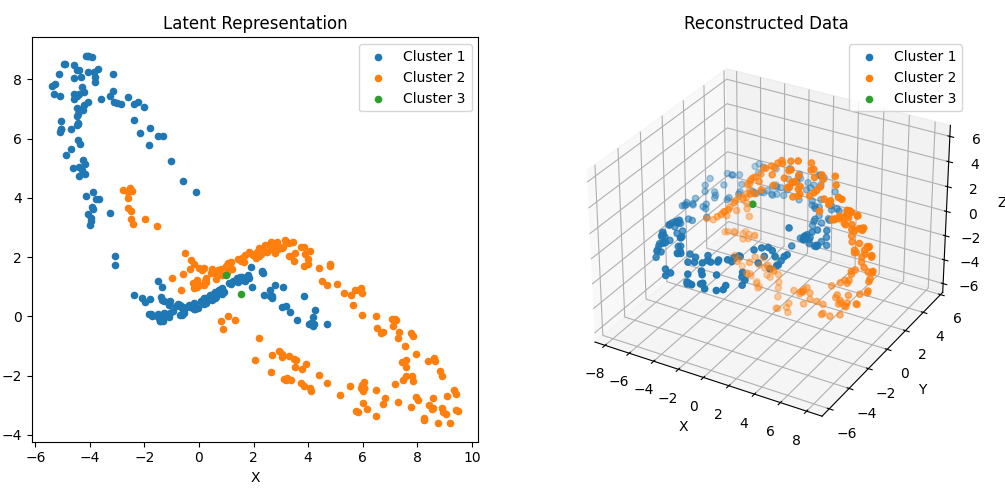
\includegraphics[width=\linewidth]{images/RQ1/3-8-4-2_0.2157.png}
    \caption{3-8-4-2 architecture with 0.2157 MSE.}
    \label{fig:3-8-4-2}
  \end{subfigure}
  \hfill
  % subfigure 4
  \begin{subfigure}[b]{0.49\textwidth}
    \centering
    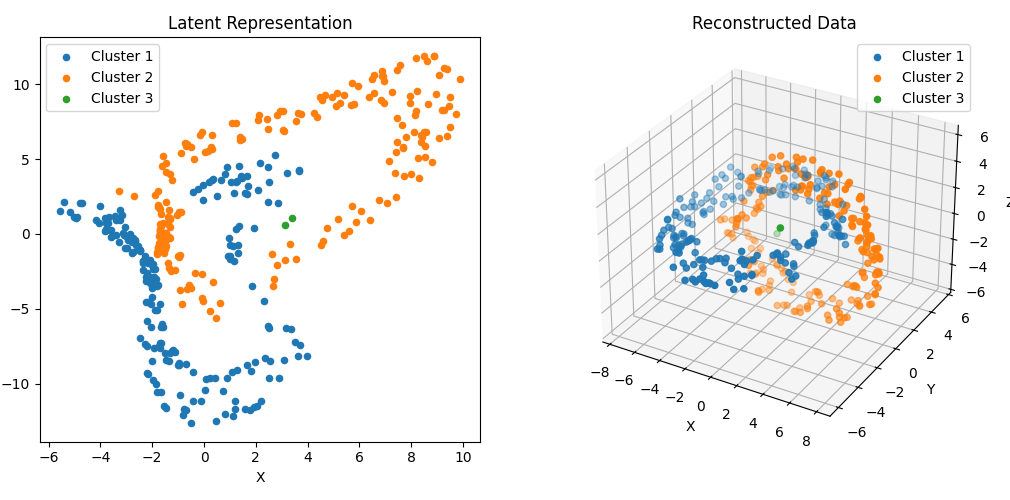
\includegraphics[width=\linewidth]{images/RQ1/3-16-8-2_0.1397.png}
    \caption{3-16-8-2 architecture with 0.1397 MSE.}
    \label{fig:3-16-8-2}
  \end{subfigure}
  \hfill  
  % subfigure 5
  \begin{subfigure}[b]{0.49\textwidth}
    \centering
    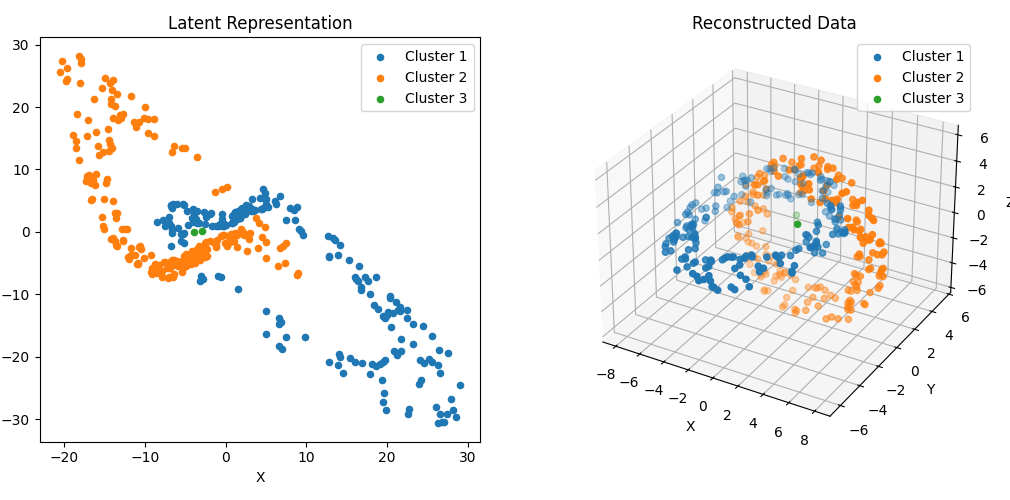
\includegraphics[width=\linewidth]{images/RQ1/3-32-16-2_0.1018.png}
    \caption{3-32-16-2 architecture with \textcolor{green!60!black}{0.1018} MSE.}
    \label{fig:3-32-16-2}
  \end{subfigure}
  \hfill  
  % subfigure 6
  \begin{subfigure}[b]{0.49\textwidth}
    \centering
    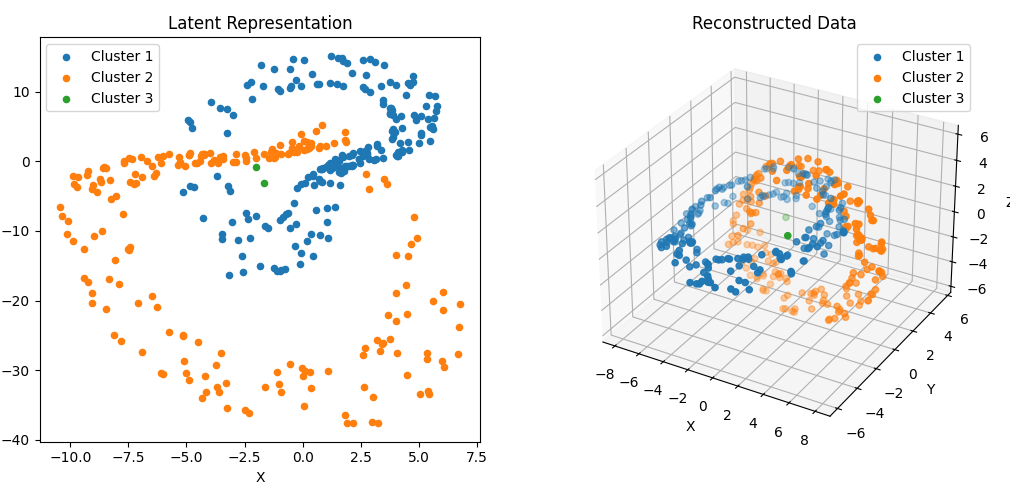
\includegraphics[width=\linewidth]{images/RQ1/3-64-32-2_0.0936.png}
    \caption{3-64-32-2 architecture with \textcolor{green!80!black}{0.0936} MSE.}
    \label{fig:3-64-32-2}
  \end{subfigure}

  \caption{Projections for 3D autoencoders with two hidden layers of varying width. 3-X-Y-2 architectures are compared.}
  \label{fig:3-X-Y-2}
\end{figure}

\begin{figure}[htb]
  \centering
  % subfigure 1
  \begin{subfigure}[b]{0.49\textwidth}
    \centering
    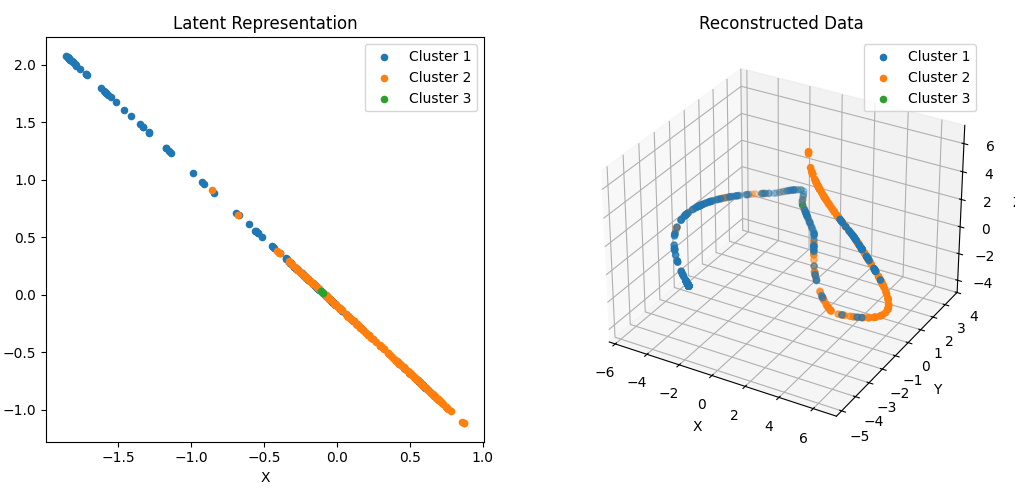
\includegraphics[width=\linewidth]{images/RQ1/3-4-2-1-2_2.1483.png}
    \caption{3-4-2-1-2 architecture with \textcolor{red!20!black}{2.1483} MSE.}
    \label{fig:3-4-2-1-2}
  \end{subfigure}
  \hfill
  % subfigure 2
  \begin{subfigure}[b]{0.49\textwidth}
    \centering
    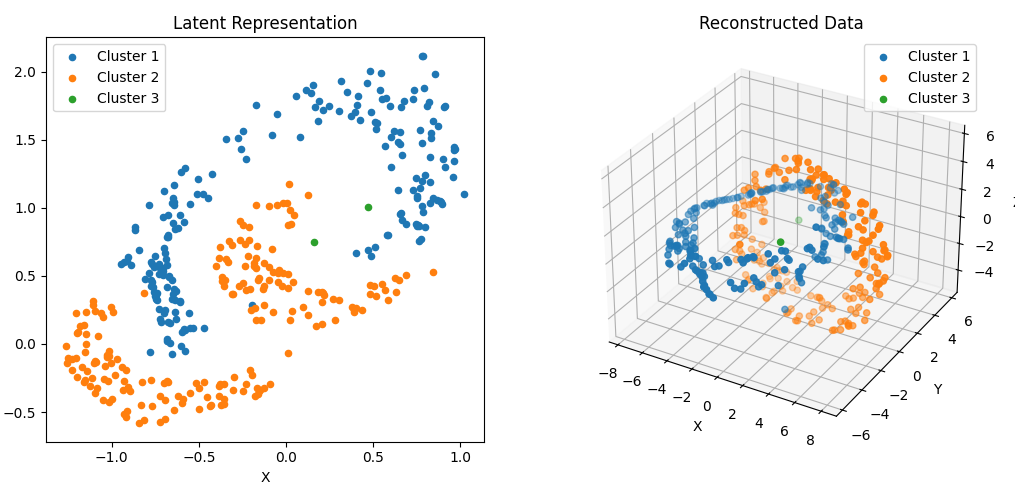
\includegraphics[width=\linewidth]{images/RQ1/3-8-4-2-2_0.2784.png}
    \caption{3-8-4-2-2 architecture with 0.2784 MSE.}
    \label{fig:3-8-4-2-2}
  \end{subfigure}
  \hfill
  % subfigure 3
  \begin{subfigure}[b]{0.49\textwidth}
    \centering
    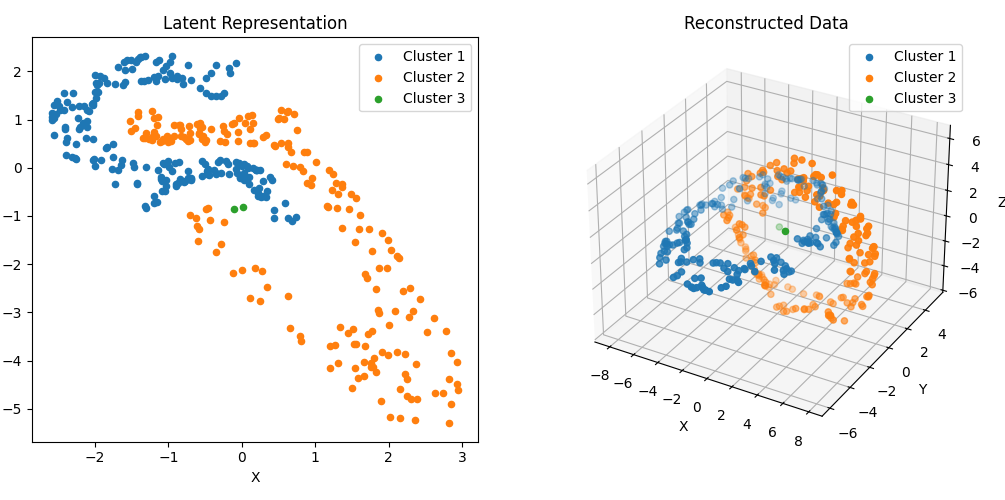
\includegraphics[width=\linewidth]{images/RQ1/3-16-8-4-2_0.1488.png}
    \caption{3-16-8-4-2 architecture with 0.1488 MSE.}
    \label{fig:3-16-8-4-2}
  \end{subfigure}
  \hfill
  % subfigure 4
  \begin{subfigure}[b]{0.49\textwidth}
    \centering
    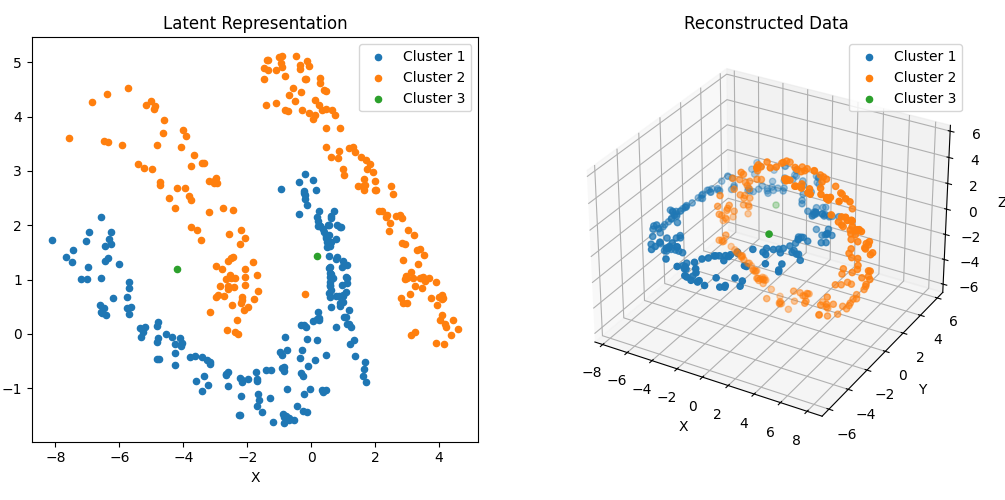
\includegraphics[width=\linewidth]{images/RQ1/3-32-16-8-2_0.1116.png}
    \caption{3-32-16-8-2 architecture with \textcolor{green!40!black}{0.1116} MSE.}
    \label{fig:3-32-16-8-2}
  \end{subfigure}
  \hfill  
  % subfigure 5
  \begin{subfigure}[b]{0.49\textwidth}
    \centering
    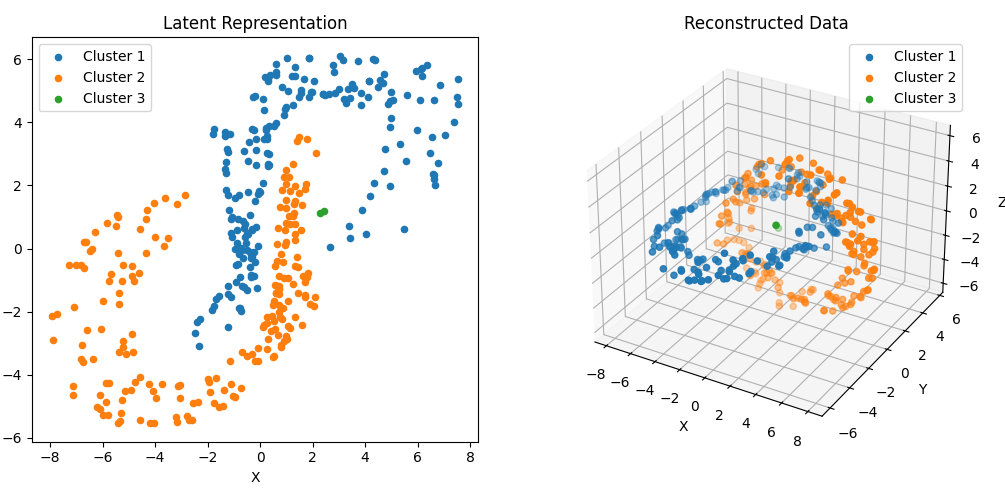
\includegraphics[width=\linewidth]{images/RQ1/3-64-32-16-2_0.0920.png}
    \caption{3-64-32-16-2 architecture with \textcolor{green!100!black}{0.0920} MSE.}
    \label{fig:3-64-32-16-2}
  \end{subfigure}
  \hfill  
  % subfigure 6
  \begin{subfigure}[b]{0.49\textwidth}
    \centering
    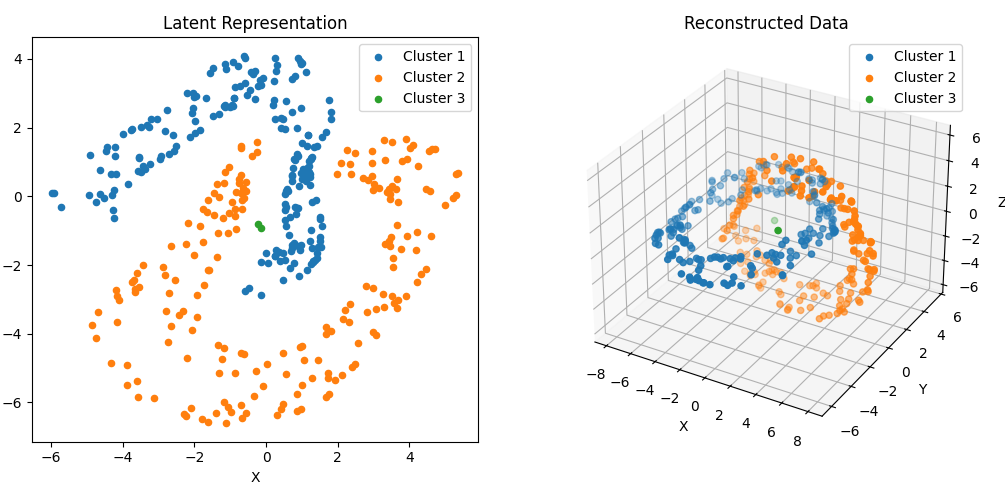
\includegraphics[width=\linewidth]{images/RQ1/3-128-64-32-2_0.1131.png}
    \caption{3-128-64-32-2 architecture with \textcolor{green!20!black}{0.1131} MSE.}
    \label{fig:3-128-64-32-2}
  \end{subfigure}

  \caption{Projections for 3D autoencoders with three hidden layers of varying width. 3-X-Y-Z-2 architectures are compared.}
  \label{fig:3-X-Y-Z-2}
\end{figure}

The first series of experiments investigated the extent to which variations in autoencoder architecture influence the preservation of in-between instances (IBIs) and cluster structures in the latent and reconstructed space. To ensure that observed effects could be attributed specifically to architectural factors, all non-structural parameters were held constant across trials. The activation function was fixed to Scaled Exponential Linear Units (SELU), optimization was performed using Adam, and the training objective consisted solely of mean squared error (MSE) reconstruction loss. A full-batch training regime was used, rendering the sampling strategy irrelevant for this set of experiments. The explanations for these choices can be read in Section \ref{sec:autoencoder_framework}.

Within this controlled setting, the architectural search focused on two key dimensions: network depth, defined as the number of hidden layers in the encoder and decoder, and network width, defined here as the number of units in the hidden layer directly before and after the bottleneck. To ensure a controlled comparison, the encoder and decoder followed a mirrored structure with a gradual reduction of neurons toward the bottleneck, in line with established architectural guidelines \cite{Charte18}. For clarity, we label only this layer when reporting “network width,” with the understanding that widths increase in powers of two toward the outer layers. For example, a label of $2^2$ denotes four neurons in the hidden layer directly before and after the bottleneck, with the number of neurons increasing exponentially toward the outer layers. This scaling approach preserves a consistent compression ratio across layers while enabling systematic variation in model capacity. It should be noted that the number of units in the input/output layers, as well as in the bottleneck layer, is ultimately constrained by the dimensionality of the dataset under consideration.

Quantitative results from the grid search are reported in Table \ref{tab:rq1-combined}, with MSE values given for each combination of depth and width, alongside the corresponding encoder configuration. In both the 2D and 3D autoencoders, the general trend indicates that increasing depth and width initially improves reconstruction performance, but gains diminish or reverse beyond a certain point. For example, in the 2D setting, the MSE decreases from 0.1449 for the baseline linear mapping (2–1 architecture, Figure \ref{fig:2-1}) to 0.0016 for a deep and moderatly wide 2–32–16–8–1 network. A similar pattern emerges in 3D, where the MSE drops from 2.1619 for the baseline linear mapping (3–2 architecture, Figure \ref{fig:3-2}) to 0.0920 for the deep and wide 3–64–32–16–2 model. However, the widest configurations, such as 2–128–64–32–1 or 3–128–64–32–2, fail to deliver further improvements and exhibit slight degradation, suggesting the onset of overfitting or instability in learning fine-grained transitional structures. This observation underscores the importance of balancing depth and width: while increased capacity enhances the expressiveness of the model and its ability to encode complex non-linear relationships, there exists a point beyond which additional layers or neurons contribute little to reconstruction quality and may in fact compromise the preservation of structural nuances in the data.

An interesting and somewhat counterintuitive observation is that the baseline linear architectures (2–1 for the 2D dataset and 3–2 for the 3D dataset) outperform the simplest nonlinear models (2–1–1 and 3–1–2) in terms of MSE. This result suggests that introducing a minimal nonlinear layer without sufficient representational capacity can, in fact, degrade reconstruction performance. In these configurations, the added nonlinearity appears to distort the mapping without providing enough hidden units to capture complex relationships, leading to both higher reconstruction error and less coherent latent structures. The linear mappings, by contrast, act as direct dimensionality-reduction operators akin to principal component analysis, preserving much of the global variance structure without introducing unnecessary transformation complexity.

The qualitative assessment of the 2D projections reinforces the trends observed in the quantitative results. For the simplest linear model 2–1 (MSE = 0.1449, Fig. \ref{fig:2-1}), the reconstructed embeddings show poor separation of clusters, with transitional regions between groups lacking clarity. As both depth and width are increased, the visual quality of the embeddings improves markedly, producing more coherent cluster shapes and smoother inter-cluster transitions. In particular, architectures such as 2–32–1 (MSE = 0.0026, Fig. \ref{fig:2-32-1}), 2–16–8–1 (MSE = 0.0017, Fig. \ref{fig:2-16-8-1}), and 2–8–4–2–1 (MSE = 0.0019, Fig. \ref{fig:2-8-4-2-1}) yield embeddings that are not only quantitatively strong but also visually well-structured. Beyond this point, further increases in width result in reconstructions that are qualitatively indistinguishable from the mentioned models. This plateau in perceived improvement is most apparent in the curvature of the reconstructed data: higher-capacity networks produce embeddings with consistently rounded, well-aligned cluster geometries, indicating that the model has fully captured the underlying manifold structure of the data.

The qualitative evaluation of the 3D autoencoder projections (Figures \ref{fig:3-2}–\ref{fig:3-X-Y-Z-2}) presents a more complex picture than in the 2D case, as the higher-dimensional latent structure is inherently harder to assess visually. The baseline linear model (3–2, MSE = 2.1619, Fig. \ref{fig:3-2}) preserves in-between instances (IBIs) relatively well, maintaining their position between the two primary toroidal clusters. However, it suffers from poor cluster separation, with the two structures appearing partially blended. Across the architectural search, the preservation of both IBIs and cluster boundaries is considerably more inconsistent than in the 2D experiments, where once a certain depth and width threshold was reached, these features were maintained reliably. 

Architectures such as 3–1–2, 3–2–1–2, and 3–4–2–1–2 (Figs. \ref{fig:3-1-2}, \ref{fig:3-2-1-2}, and \ref{fig:3-4-2-1-2}) lack sufficient representational capacity due to having a hidden layer with width = 1, effectively collapsing the embedding into a one-dimensional manifold. This loss of dimensionality severely limits the model’s ability to reconstruct the original 3D topology. 
Slightly larger configurations such as 3–2–2 and 3–4–2–2 (Figs. \ref{fig:3-2-2} and \ref{fig:3-4-2-2}) avoid this collapse but still fail to achieve clear cluster separation, resulting in intertwined or partially overlapping structures.
Other architectures, including 3–4–2, 3–16–2, 3–8–4–2–2, and 3–32–16–8–2 (Figs. \ref{fig:3-4-2}, \ref{fig:3-16-2}, \ref{fig:3-8-4-2-2}, and \ref{fig:3-32-16-8-2}), exhibit another form of distortion, with certain clusters appearing unusually torn apart, fragmenting their geometric continuity. 
A distinctive “yin–yang” pattern emerges in configurations such as 3–8–2, 3–8–4–2, 3–32–16–2, 3–64–32–2, 3–16–8–4–2, 3–64–32–16–2, and 3–128–64–32–2 (Figs. \ref{fig:3-8-2}, \ref{fig:3-8-4-2}, \ref{fig:3-32-16-2}, \ref{fig:3-64-32-2}, \ref{fig:3-16-8-4-2}, \ref{fig:3-64-32-16-2}, and \ref{fig:3-128-64-32-2}), where both clusters open in such a way that portions of each curve around the other, effectively allowing one cluster to pass through the other in latent space. While visually striking, this geometry does not necessarily correspond to improved IBI representation, as the transitional points may be displaced along these openings. In fact, perfect IBI preservation, defined here as IBIs being positioned centrally between the two tori without a noticeable shift toward either cluster, is observed only in a subset of configurations: 3–2–2, 3–8–2, 3–16–2, 3–32–2, 3–4–2–2, 3–32–16–2, 3–64–32–2, and 3–128–64–32–2 (Figs. \ref{fig:3-2-2}, \ref{fig:3-8-2}, \ref{fig:3-16-2}, \ref{fig:3-32-2}, \ref{fig:3-4-2-2}, \ref{fig:3-32-16-2}, \ref{fig:3-64-32-2}, and \ref{fig:3-128-64-32-2}). These architectures successfully maintain the intended spatial relationships, but the surrounding structural variations highlight that, in 3D, achieving consistent preservation of both cluster integrity and in-between structure is considerably more challenging than in the 2D case.
\newline

A notable distinction between the 2D and 3D experiments is the relationship between IBI preservation and reconstruction error. In the 2D case, there is a clear correlation: models that achieve lower MSE values also tend to produce latent embeddings in which inter-cluster regions are geometrically coherent and IBIs occupy positions that align well with the corresponding definition. In other words, as a rule of thumb for the 2D setting, higher-capacity architectures not only reduce reconstruction error but also maintain the spatial plausibility of in-between regions and clusters, making visual inspection a reliable complement to quantitative evaluation. By contrast, this relationship breaks down in the 3D experiments. Here, low MSE values do not consistently coincide with high-quality IBI and cluster preservation. Several models with strong reconstruction performance exhibit distortions in cluster topology or misplacement of transitional points, while certain architectures with higher MSE still preserve these structures satisfactorily. This inconsistency suggests that, in 3D, IBI fidelity is not necessarily dependent on network depth and width once a certain minimum capacity threshold has been reached. Consequently, while MSE remains a useful guide for identifying adequately expressive architectures, the accompanying visualizations in 3D are less decisive for verifying that in-between structure is preserved. 

Based on these observations, the models selected for further experiments and subsequent research questions are those with the best MSE performance in their respective dimensional settings: 2–32–16–8–1 (Fig. \ref{fig:2-32-16-8-1}) for the 2D datasets and 3–64–32–16–2 (Fig. \ref{fig:3-64-32-16-2}) for the 3D datasets. These configurations offer the most effective compromise between expressive power and the risk of overfitting, while ensuring that the learned representations are well-suited for the subsequent loss-functions and supervision analyses.
